\section{Эксперимент}
\label{sec:Chapter5} \index{Chapter5}

\subsection{Описание эксперимента}

%Постановка эксперимента. Что планируется сделать и какие результаты хочется получить. Какие метрики будем использовать и по каким метрикам будем сравнивать.

В рамках данного исследования было решено провести эксперимент по адаптации моделей распознавания ключевых точек на теле человека к целевому набору данных. В представленном разделе будет рассказано про выбранные модели, алгоритм доменной адаптации, описание исходного и целевого наборов данных и метрик оценивания результатов работы нейронных сетей.

\subsubsection*{Выбор модели для эксперимента}

Многие модели из представленных в \autoref{sec:Chapter4} были представлены в рамках проекта MMPose, что значительно облегчило эксперимент с точки зрения подготовки пайплайнов предобработки данных и построения конфигураций нейронных сетей. Также критерием отбора стала возможность обучения модели в условиях ограниченных вычислительных ресурсов, так как адаптация проводилась в рамках платформы Google Colab. В итоге было выбрано 4 (МОЖЕТ БЫТЬ 3) модели:
\begin{enumerate}
\item HRNet
\item ViTPose
\item RTMPose
\item SimCC + ResNet
\end{enumerate}

Выбранные модели будут обучены на исходном домене в течении 20 эпох. От этого состояния будет начинать при проведении адаптации.

\subsubsection*{Описание метода доменной адаптации}

В рамках эксперимента будет оптимизирован метод Progressive Unsupervised Learning \cite{pul} для задачи распознавания ключевых точек. 

Основной сложностью выступает выбор функции фильтрации невалидных результатов. И в рамках эксперимента предлагается использовать фильтрацию по уровню уверенности модели в предсказанной ключевой точке. Средняя уверенность полученных из предсказания результатов для одного изображения будет сравниваться с заранее заданным пороговым значением. Все значения, перешедшие этот порог попадают в псевдо-обучающую выборку.

Заметим, что для точек, которые не являются видимыми, уверенность сильно меньше, что может портить среднюю уверенность для фотографии. Таким образом получаем ещё одну функцию фильтрации - по средней уверенности для видимых точек результата.

На каждой итерации будет проводиться дообучение модели в течение 10 эпох. Количество итераций будет ограничено либо сходимостью метрики качества, либо количеством 10 штук.

\subsubsection*{Метрики оценки качества распознавания}

Для проведения количественной оценки работы алгоритма во всех случаях необходимо использовать метрики оценки предсказания. Выбранные метрики дают полную оценку того, насколько хорошо модель работает, как с точки равнозначности всех точек в топологии, так и с учетом их веса в скелете.

\begin{enumerate}
\item Percentage of Correct Keypoints

Первой рассмотрим метрику PCK, которая равнозначно воспринимает все ключевые точки. Для нее важно попало ли предсказания в окрестности реального результата, причем размер окрестности может быть выбран как фиксированный для всего тестового набора, так и зависеть от высоты человека на изображении. Математическую формулу метрики можно представить в следующем виде:

\begin{equation}
	PCK = \frac{\sum_{i=1}^{n} bool(d_i < threshold * body\_height)}{n},
\end{equation}
	
где $d_i$ - расстояние между предсказанной и правильной точкой,\\
$threshold$ - порог, задаваемый исследователем,\\
$body\_height$ - высота прямоугольника, внутри которого находится человек,\\
$bool(*)$ - логическое условие, возвращает 1, если оно верно и 0 в ином случае,\\
$n$ - размер выборки.

\item Object Keypoint Similarity

OKS была представлена для оценки решений задачи распознавания ключевых точек в рамках соревнования COCO \cite{COCO_topology}. Авторы старались провести аналогию с метрикой Intersection over Union (IoU) для задачи детекции объектов, чтобы можно было пользоваться метрикой average precision, о которой будет рассказано далее.

В отличие от предыдущей метрики, OKS не считает все точки равнозначными. Для этого проводится процедура нормализации расстояния между предсказанной и реальной точками. Одним из шагов нормализации является учет размера детектируемого объекта, что показывает различия для детекции скелета людей на заднем и переднем планах. Вторым шагом нормализации является учет дисперсии данной ключевой точки.

\hfill

Математическая формула метрики выглядит следующим образом:

\begin{equation}
	OKS = \frac{\sum_{i} exp\left( - d_i^2 / 2s^2k_i^2\right)\delta\left(v_i > 0\right)}{\sum_{i} \delta\left(v_i > 0\right)},
\end{equation}

где $d_i$ - расстояние между предсказанной и правильной точкой,\\
$s$ - масштаб объекта,\\
$k_i$ - константа ключевой точки, контролирующая спад,\\
$v_i$ - видимость точки по аннотации COCO, где 0 обозначает, что точка не была размечена.

\item Average Precision

AP - метрика, широкоиспользуемая для оценки качества моделей в задача классификации и обнаружения объектов. Она измеряет точность нейронной сети, принимая во внимание как ее способность правильно классифицировать объекты, так и ее способность точно их локализовать.

Исходя из названия метрика использует такие понятие как Precision, показывающее доли правильно предсказанных положительных примеров среди всех положительно предсказанных результатов, и Recall, показывающее долю правильно предсказанных положительных примеров среди всех фактических положительных примеров.
$$
Precision = \frac{TP}{TP + FP} \text{, } Recall = \frac{TP}{TP + FN}
$$
При использовании OKS верно положительным результатом является тот, для которого метрика OKS больше заданного порогового значения. Неверно положительными являются те результаты, метрика OKS для которых не перешла заранее заданный порог. Неверно отрицательными являются все реальные данные, для которых результата получено не было.
$$
TP\text{ при }OKS > threshold\text{ и }FP\text{ при }OKS \leq threshold
$$
Используя описанные пояснения можно рассчитать значения метрик точность и полнота. С их помощью строится кривая precision-recall, которая показывает изменения точности в зависимости от полноты. Площадь под ее графиком и будет являться значением метрики AP. Часто она высчитывается интегрирования кривой precision-recall методом трапеций, который показан на \autoref{fig:trapz}.

\begin{figure}[h]
	\centering
	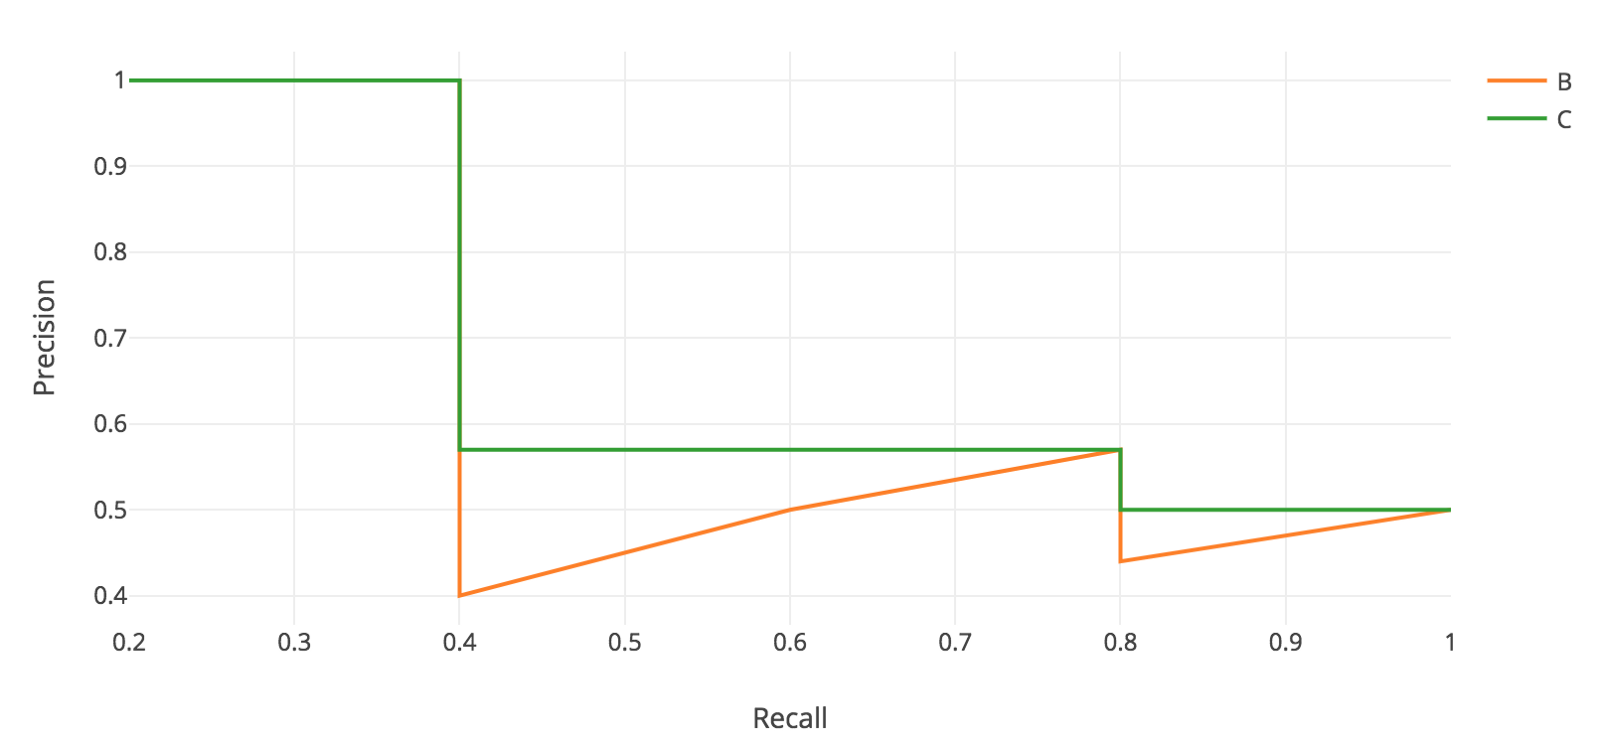
\includegraphics[width=.75\textwidth]{./images/AP}
	\caption{Применения метода трапеций для интегрирования кривой precision-recall.}
	\label{fig:trapz}
\end{figure}

Для задачи детекции обычно применяется несколько порогов: $AP^{0.5}$, $AP^{0.75}$ и $AP = mAP = mean AP^{0.5:0.05:0.95}$.

\end{enumerate}

\subsection{Данные}

По условиям задачи доменной адаптации необходимо найти два набора данных для эксперимента. Далее приведем информацию о выбранных доменах и их характеристиках.

\subsubsection*{Исходный домен}

В качестве исходного домена выбран набор данных Common Objects in Context \cite{COCO_dataset}. COCO — это крупный датасет, широко используемый в области компьютерного зрения для задач распознавания объектов, сегментации, и создания описательных подписей к изображениям. Он был создан Microsoft и с тех пор стал стандартом для обучения и оценки алгоритмов компьютерного зрения.

\begin{figure}[h]
	\centering
	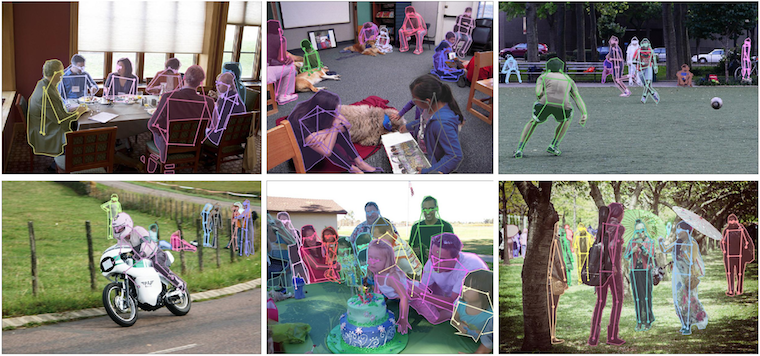
\includegraphics[width=\textwidth]{./images/data_info/coco_dataset}
	\caption{Примеры изображений из набора данных COCO. \cite{COCO_topology}}
	\label{fig:coco_dataset}
\end{figure}

Учитывая, что в рамках соревнований COCO была и задача детекции ключевых точек (Keypoint detection) \cite{COCO_topology}, то часть этого набора данных была размечена под нее. Если быть точным, то датасет включает более 250 тысяч аннотаций людей на различных изображениях. Формат аннотаций включает в себя:

\begin{enumerate}

\item \textit{id} - уникальный номер аннотации;

\item \textit{image\_id} - уникальный номер изображения, которому принадлежит данная аннотация;

\item \textit{category\_id} - уникальный номер категории, к которой относится данная аннотация. Для задачи оценки позы везде выставляется категория person;

\item \textit{keypoints} - массив из 17 ключевых точек, для каждой их которых указаны координаты (x, y) на изображении, а также информация о видимости. Точки, которые не представлены на изображении заполняются нулями;

\item \textit{num\_keypoints} - здесь содержится информация о количестве размеченных точек для данной аннотации;

\item \textit{bbox} - информация об ограничивающем человека прямоугольнике. Значения внутри лежат в следующем формате: $[x, y, width, height]$;

\item \textit{area} площадь сегментированного человека. Значение необходимо при высчитывании метрики OKS;

\item \textit{iscrowd} - информация о том, одиночный человек представлен на изображении или толпа людей.

\end{enumerate}

Также в рамках задачи Keypoint Detection была введена метрика OKS и метрика mAP, о которых было рассказано ранее. Они представляют собой единые критерии для оценки моделей, что облегчает сравнение и улучшение результатов различных алгоритмов, поэтому регулярно используются для оценки  новых методов и технологий.

В рамках задачи были выбраны 8000 аннотаций, которые содержат все 17 ключевых точек то топологии COCO. На них и было произведено обучение моделей для получения бейзлайнов эксперимента.

\subsubsection*{Целевой домен}

%Описание собранных данных. Численный объем датасета. Возможно количество локаций и распределение по ним.

%Необходимо предоставить данные по распределению данных между людьми, по количеству данных для обучения/тестирования. Предоставить данные по локациям. Предоставить картинки с примерами данных, которые были собраны.

%Описание системы полуавтоматической разметки данных. Что там использовалось и как проходит разметка.

В качестве целевого набора данных был собран отдельный набор данных боксеров. В наборе данных представлены 2 человека, снятые с 3 ракурсов: профиль, анфас и 3/4. Датасет состоит из 10 видеозаписей, которые содержат порядка 10 тысяч кадров. Для проведения эксперимента выбрано 2,6 тысячи изображений, которые были впоследствие размечены. Из них для тестовой выборки отобрано около 420 изображений, а оставшиеся 2200 составили обучающую выборку, на которой и проводилась адаптация.

\begin{figure}[h]
\begin{subfigure}[b]{0.24\textwidth}
	\centering
	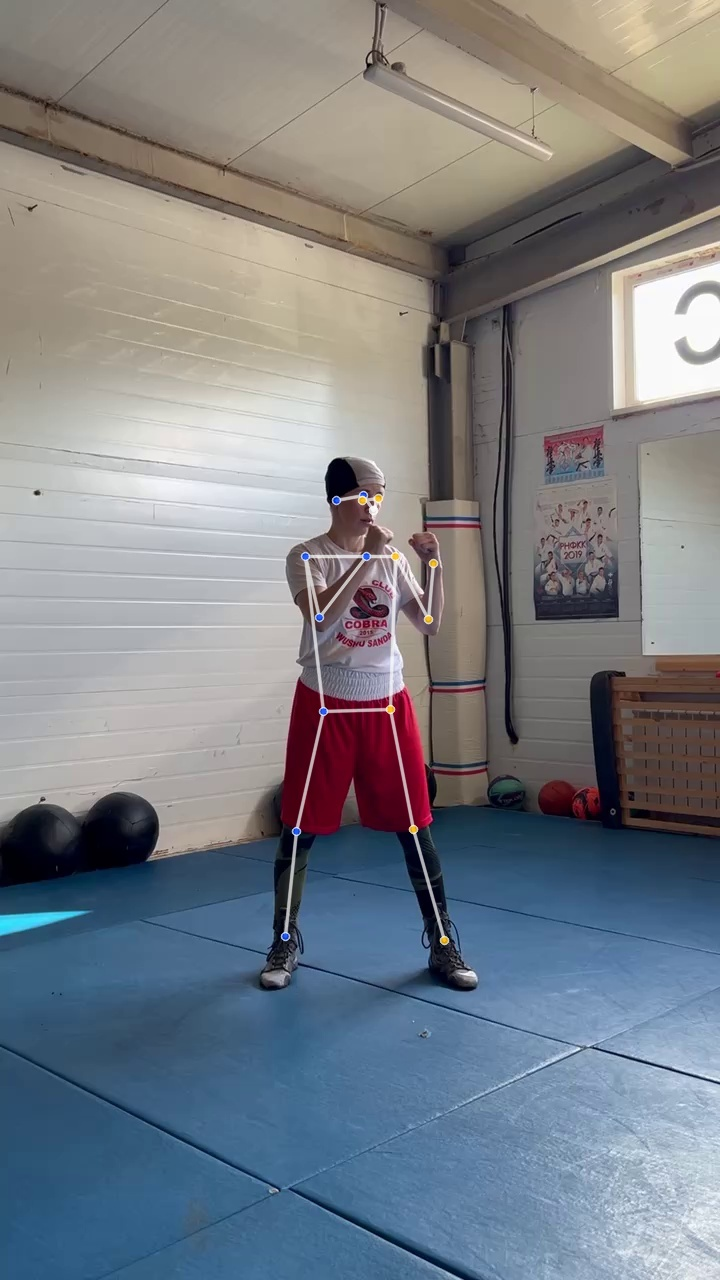
\includegraphics[width=\textwidth]{./images/data_info/box_examples/ex_5}
\end{subfigure}
\begin{subfigure}[b]{0.24\textwidth}
	\centering
	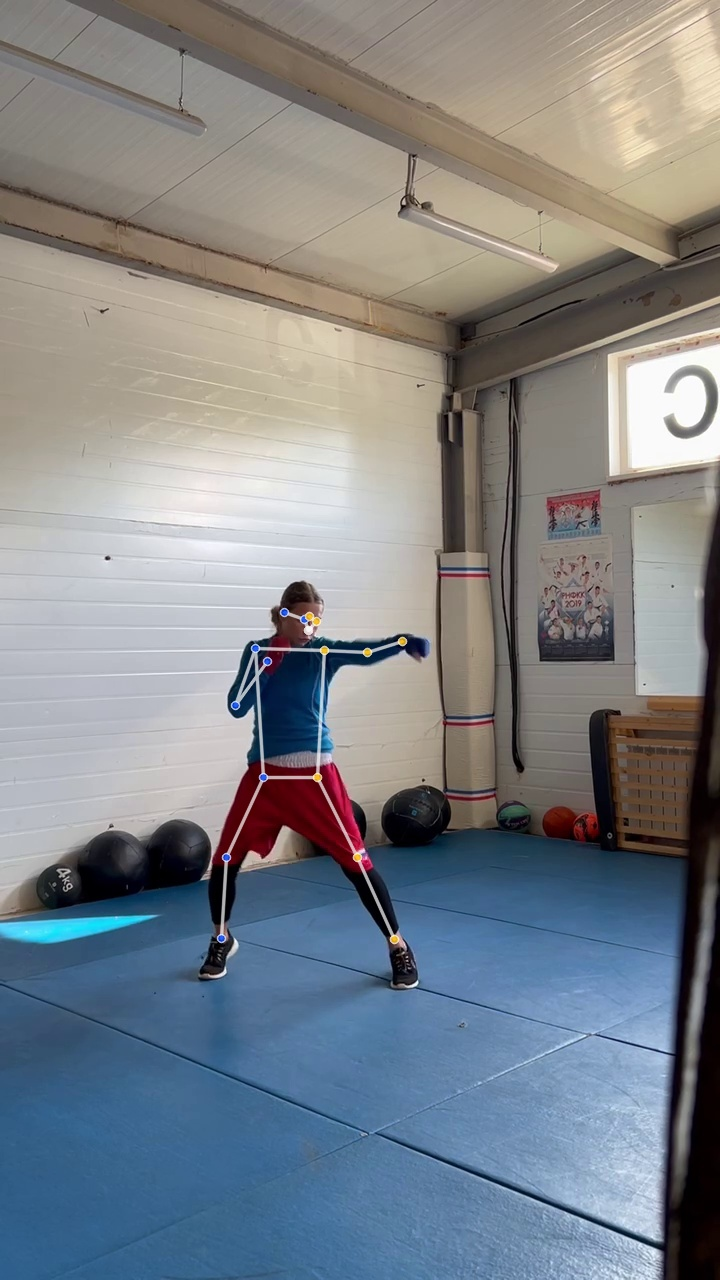
\includegraphics[width=\textwidth]{./images/data_info/box_examples/ex_1}
\end{subfigure}
\begin{subfigure}[b]{0.24\textwidth}
	\centering
	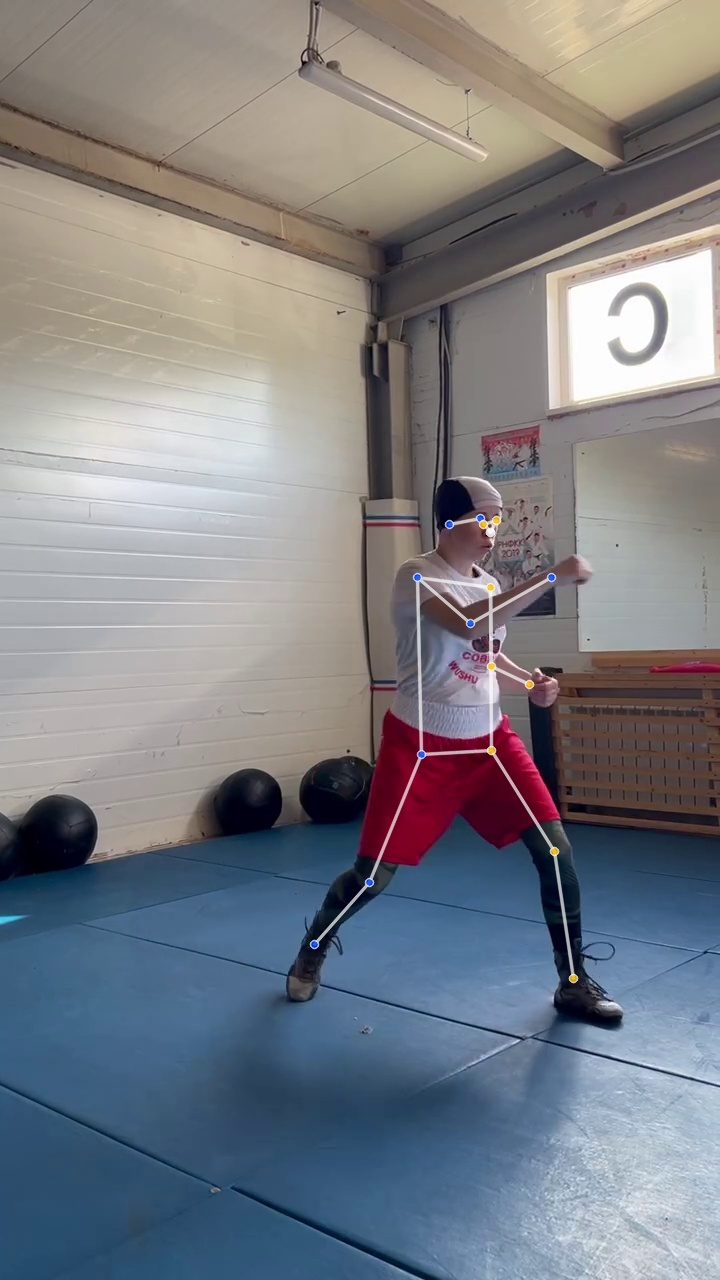
\includegraphics[width=\textwidth]{./images/data_info/box_examples/ex_9}
\end{subfigure}
\begin{subfigure}[b]{0.24\textwidth}
	\centering
	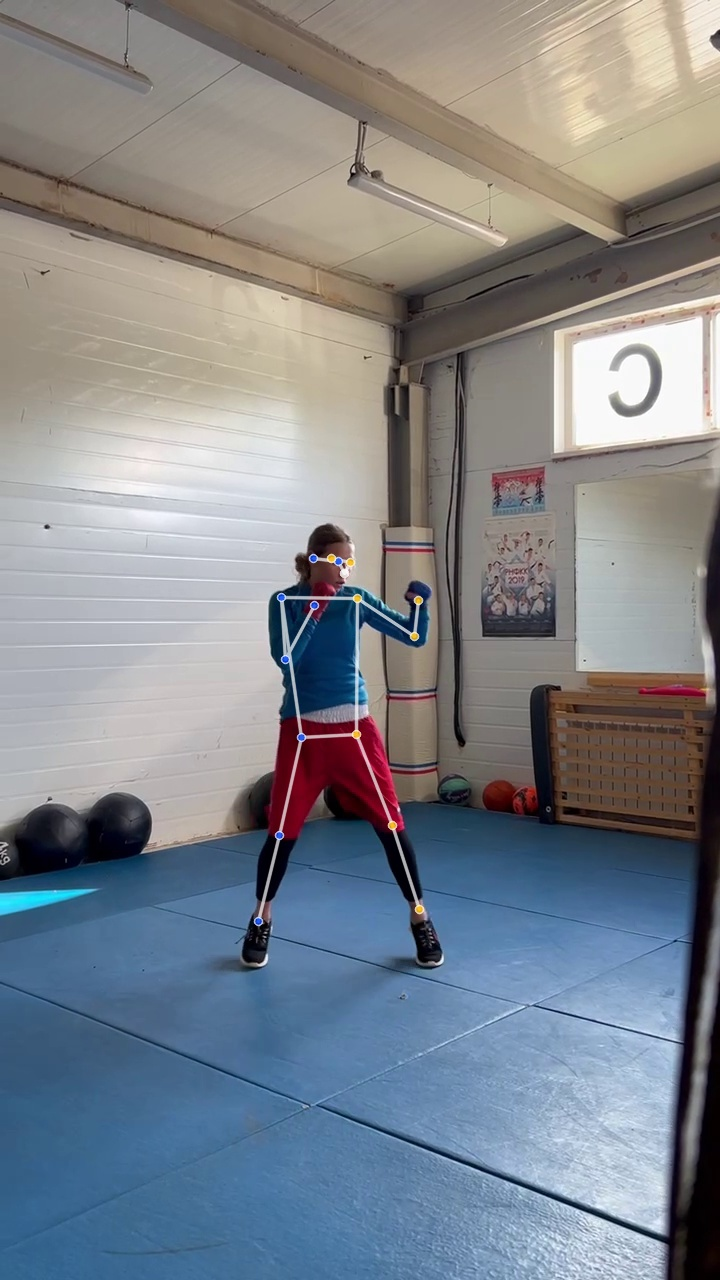
\includegraphics[width=\textwidth]{./images/data_info/box_examples/ex_0}
\end{subfigure}
\caption{Примеры изображений целевого домена.}
\label{fig:target_examples}
\end{figure}

В рамках задачи по аннотированию собранных данных была разработана система полуавтоматической разметки изображений pose-markup \cite{pose_markup}. Она представляет собой предобученную модель распознавания ключевых точек и инструмент для визуальной корректировки данных экспертом.

Для автоматической части использовалась модель BlazePose от проекта MediaPipe \cite{mediapipe}. Выбор сделан благодаря высоким характеристикам скорости инференса результатов и их точности у данного решения. А также для того, чтобы избежать корреляции размеченных данных с предсказаниями, которые будут оцениваться в рамках эксперимента. Результат, возвращаемый моделью был преобразован к формату аннотаций COCO, который был описан выше и сохранен в формате JSON. 

\begin{figure}[h]
\begin{subfigure}[b]{0.32\textwidth}
	\centering
	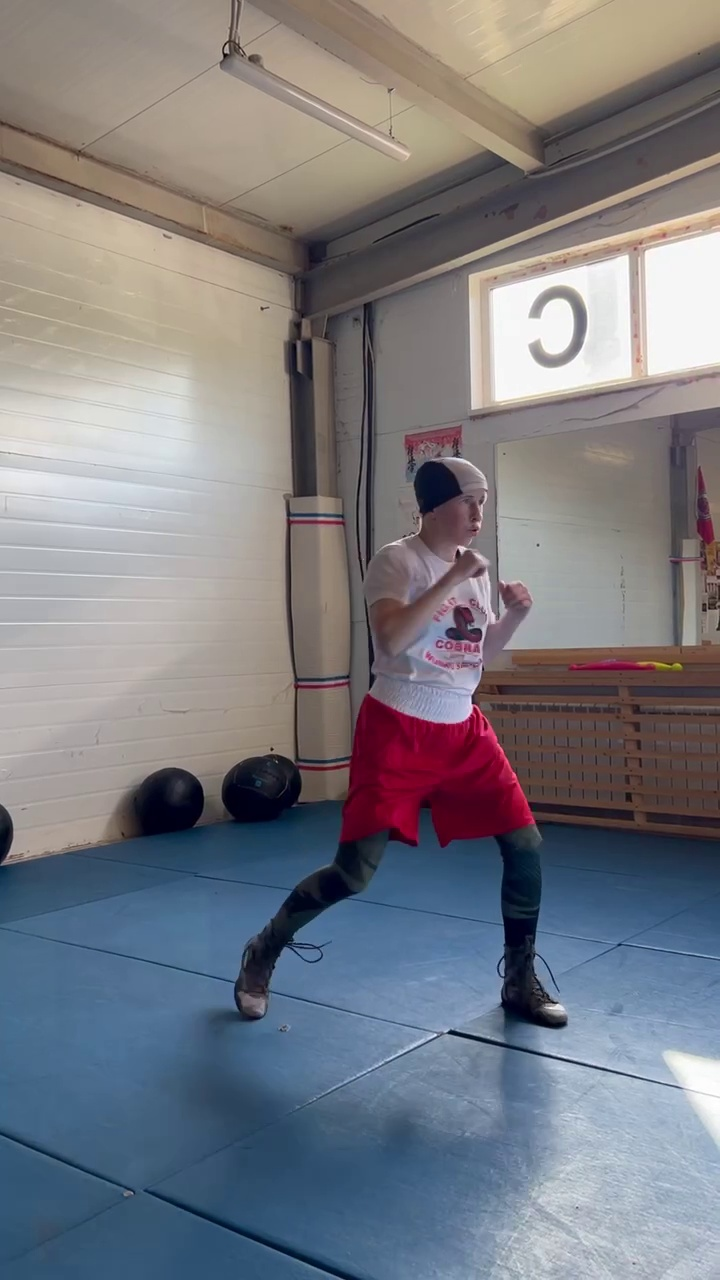
\includegraphics[width=\textwidth]{./images/data_info/pose_markup_examples/raw}
	\caption{Изначальное изображение}
\end{subfigure}
\begin{subfigure}[b]{0.32\textwidth}
	\centering
	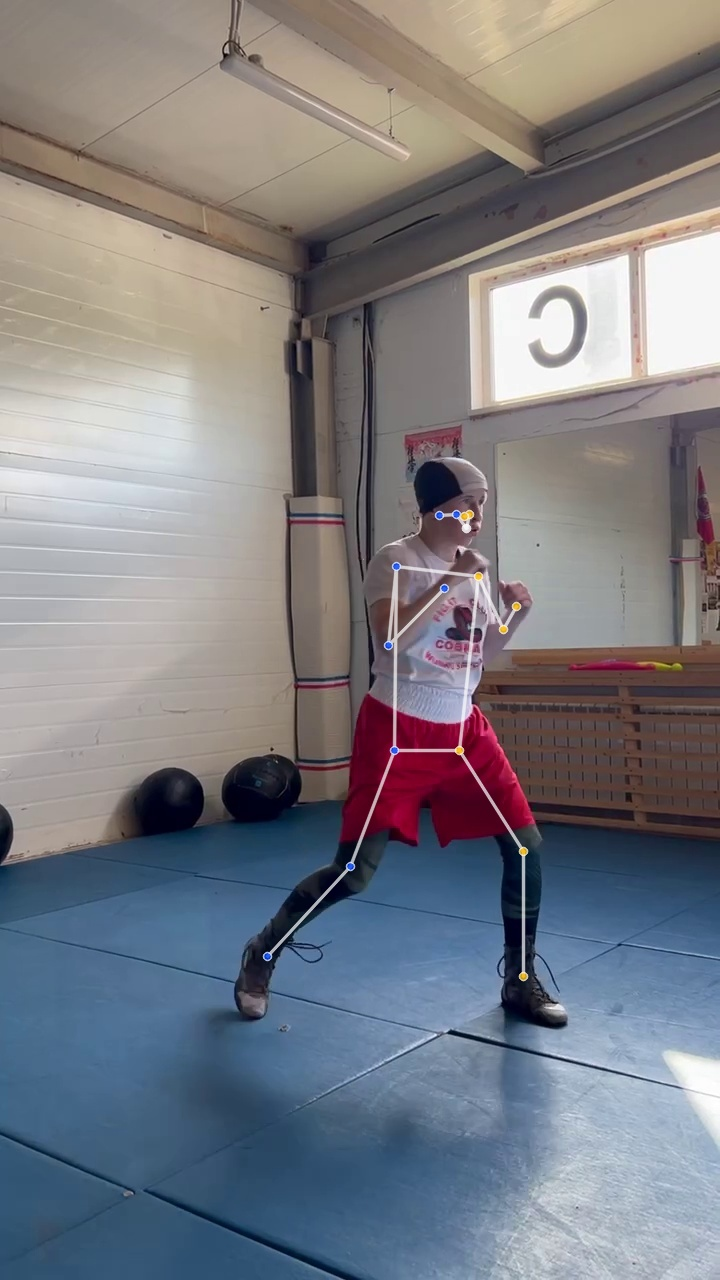
\includegraphics[width=\textwidth]{./images/data_info/pose_markup_examples/auto_labeled}
	\caption{После автоматической разметки}
\end{subfigure}
\begin{subfigure}[b]{0.32\textwidth}
	\centering
	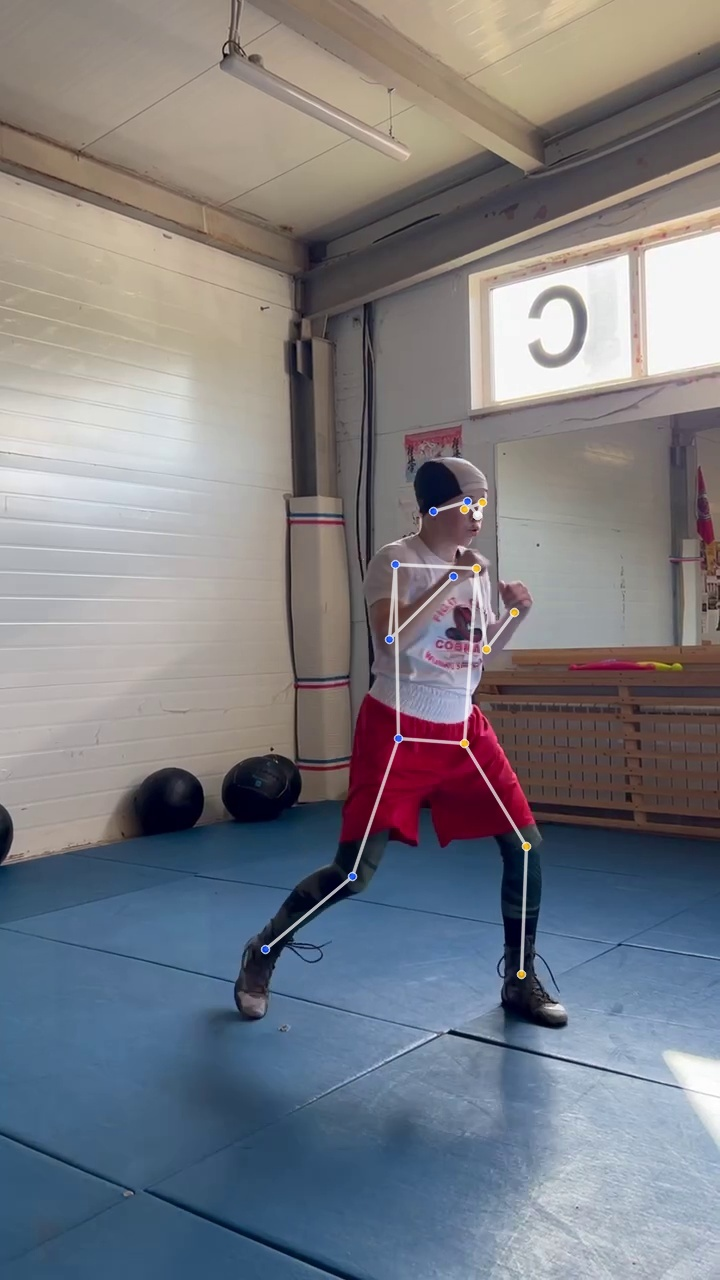
\includegraphics[width=\textwidth]{./images/data_info/pose_markup_examples/correct_labels}
	\caption{После корректировки экспертом}
\end{subfigure}
\caption{Пример работы системы полуавтоматической разметки данных.}
\label{fig:pose_markup_example}
\end{figure}

Как можно видеть на \autoref{fig:pose_markup_example}, модель имеет неточности, которые необходимо было исправить эксперту. Для этой цели использовалась вторая часть программы - инструмент для визуальной корректировки данных экспертом. 

Проанализировав результаты внесенных изменений, получили, что каждый кадр требовал правки ключевых точек. Средние показатели изменений на кадр:

\begin{itemize}
\item Собирая статистику любых изменений в точках, даже сдвига на соседний пиксель, получаем, что в среднем 14.9 точек на кадре были изменены. Распределение этих исправлений по топологии представлено на \autoref{fig:any_correction}.
\item Если считать точки, которые были значительно сдвинуты (5 и более пикселей), то их в среднем приходилось 6.5 на кадр. Большинство из них были сосредоточены на лице и левой конечности человека. Более детальное распределение изменений по топологии представлено на \autoref{fig:big_correction}.
\end{itemize}

\begin{figure}[h]
\centering
\begin{subfigure}[b]{0.4\textwidth}
	\centering
	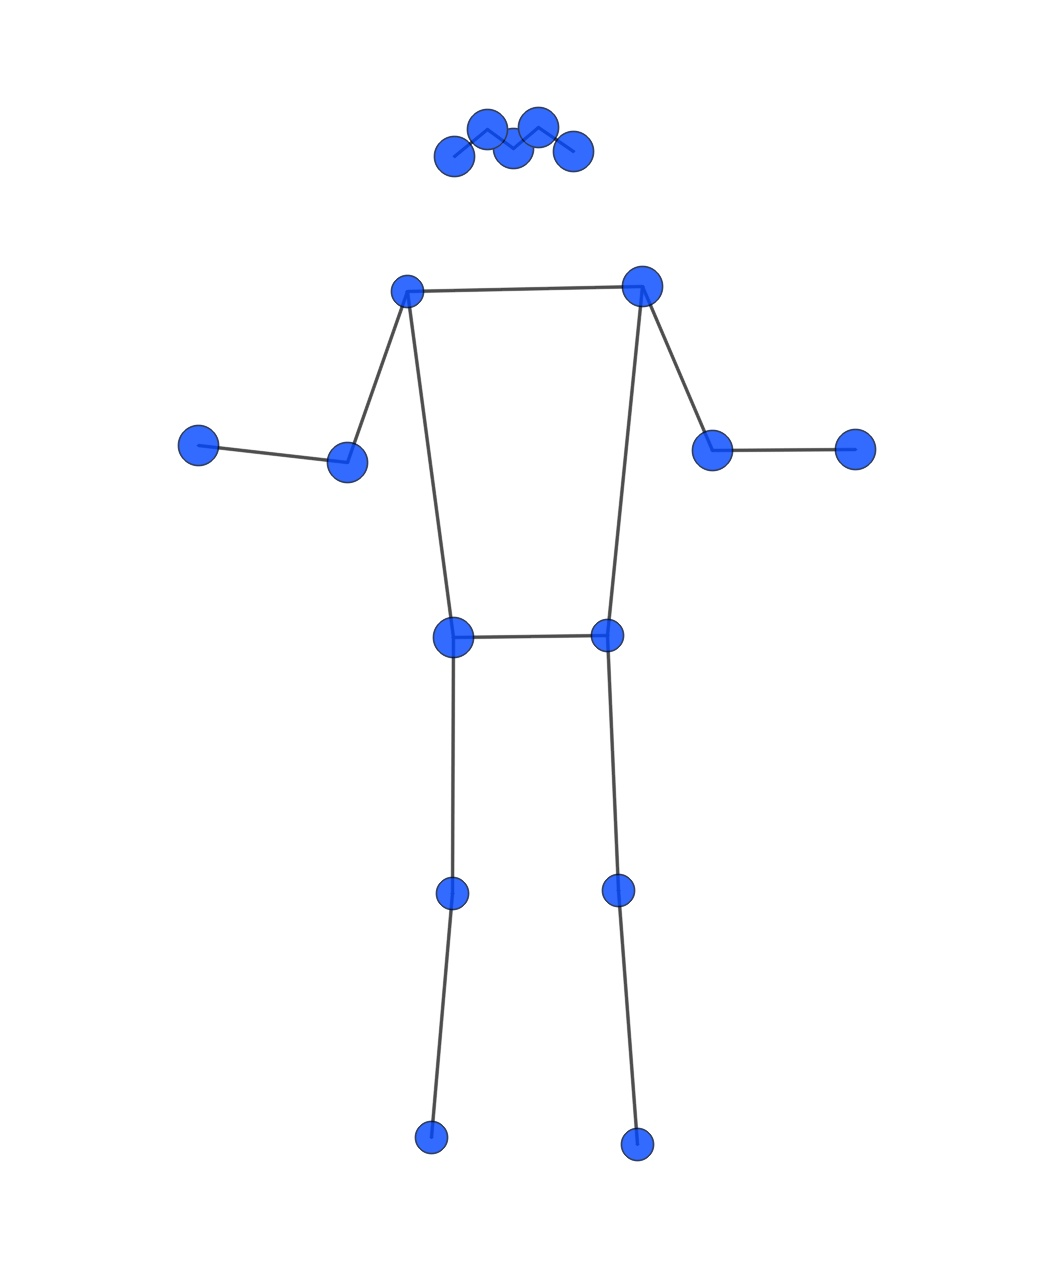
\includegraphics[width=\textwidth]{./images/data_info/pose_markup_examples/change_percentage}
	\caption{}
	\label{fig:any_correction}
\end{subfigure}
\begin{subfigure}[b]{0.4\textwidth}
	\centering
	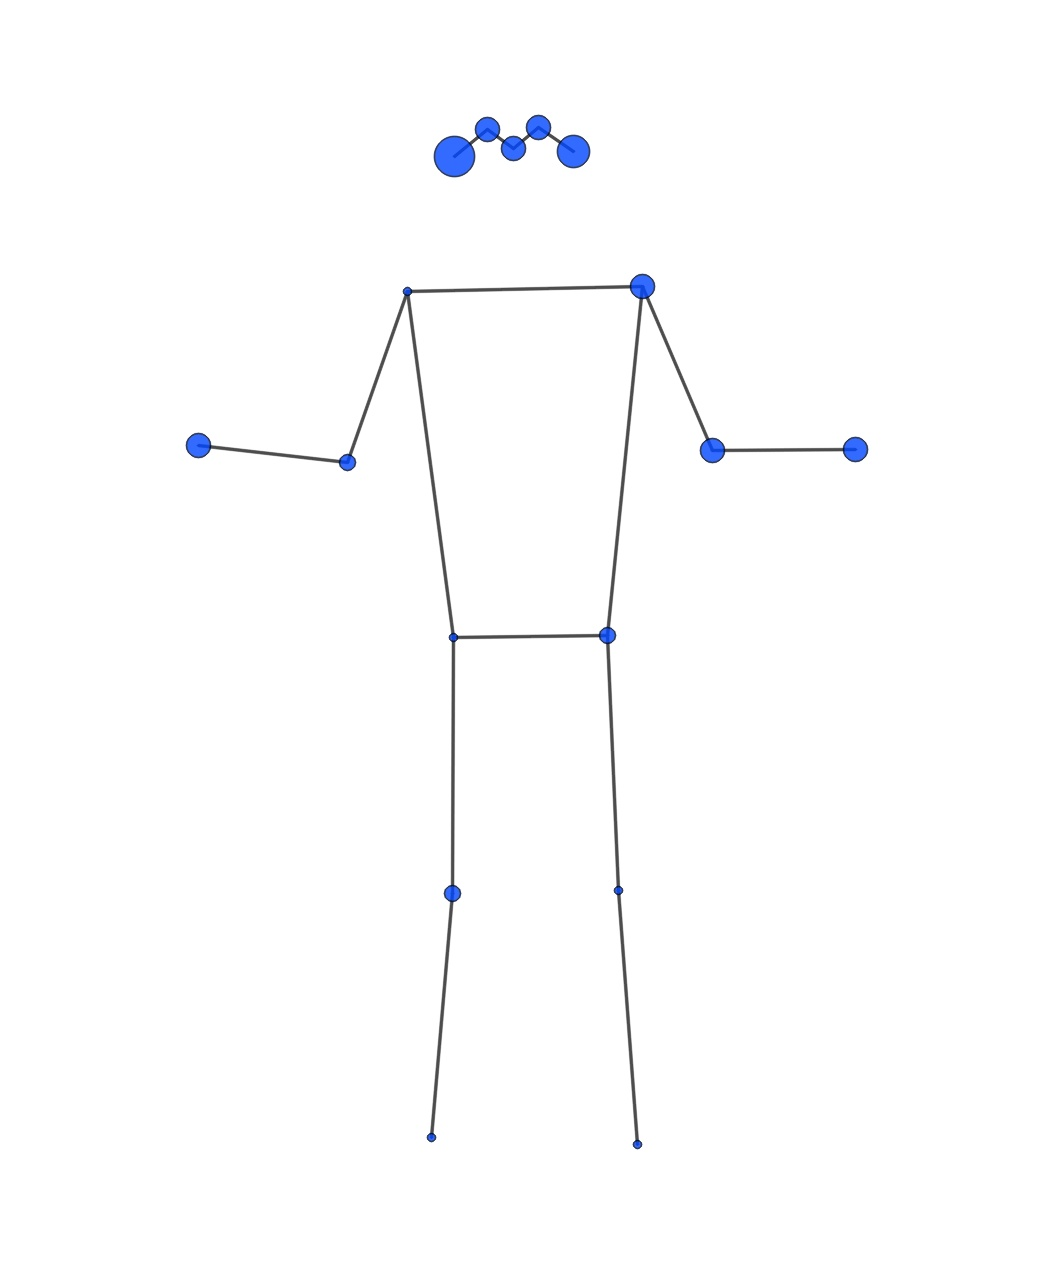
\includegraphics[width=\textwidth]{./images/data_info/pose_markup_examples/big_change_percentage}
	\caption{}
	\label{fig:big_correction}
\end{subfigure}
\caption{Схематическое представление изменений в точках, внесенных экспертом.}
\label{fig:correction_heatmap}
\end{figure}

\subsection{Результаты эксперимента}

%Тут можно сказать про ресурсы и про то, какие постановки эксперимента будут сделаны.

%Предоставить относительно сухо результаты эксперимента. Можно дать базовый анализ ситуации и того, что мы видим.

%Необходимо предоставить результаты по времени обучения нейросетей, времени дообучения нейросетей. 
%Собрать данные по количеству ошибок до-после обучения. Собрать данные по количеству ошибок при изменении домена. 
%Данные по ресурсам, на которых обучались нейросетки.


В рамках эксперимента для выбранных ранее моделей был применен алгоритм доменной адаптации PUL, который показал смешанные результаты на разных архитектурах. Для алгоритма необходимо было выбрать порог уверенности, по которому будет фильтроваться псевдо-разметка. Так как в течении первых итераций адаптации уверенность модели в результатах падала, то и размер псевдовыборки падал до нулля при высоких значениях порогового значения. Исходя из этого для каждой конкретной нейронной сети порог подбирался персонально. Влияние этого фактора будет оценено позднее.

%МНЕ КАЖЕТСЯ, ЧТО СЛЕДУЮЩИЙ АБЗАЦ НЕ ОЧЕНЬ ИНФОРМАТИВЕН.

%Отфильтрованная на каждой итерации выборка разделялась на обучающую и валидационную. На последней из них бралось значение метрики PCK, которое служило оценкой обучения модели к псевдо раззметкам. Графики зависимости предсказанных уровней будут дополнительно предоставлены.

Тестирование моделей производилось с использованием графического ускорителя NVIDIA MX250 с 2 Гб памяти. Так как объемов памяти этого ускорителя не хватало для обучения моделей, для обучения моделей была соверешена миграция в облачный сервис Google Colab с использованием предоставляемого там графического ускорителя NVIDIA Tesla T4 с 16 Гб памяти.

НАДО СКАЗАТЬ, ЧТО МОДЕЛЬ БУДЕТ СРАВНИВАТЬСЯ С ДООБУЧЕННОЙ НА ВСЕМ ЦЕЛЕОМ ДОМЕНЕ ВЕРСИЕЙ СЕБЯ.

\subsubsection*{HRNet}

С учетом того, что базовая сеть была не уверена в предсказываемых ее результатах, confidence\_threshold был выбран равным 0,4. В связи с этим для итеративных процессов отбирались данные, которые не являлись точными. В связи с этим модель показывала все более плохие результаты с каждой новой итерацией. График метрики PCK на целевом домене представлен на \autoref{fig:hrnet_pck}. 

\begin{figure}[h]
	\centering
	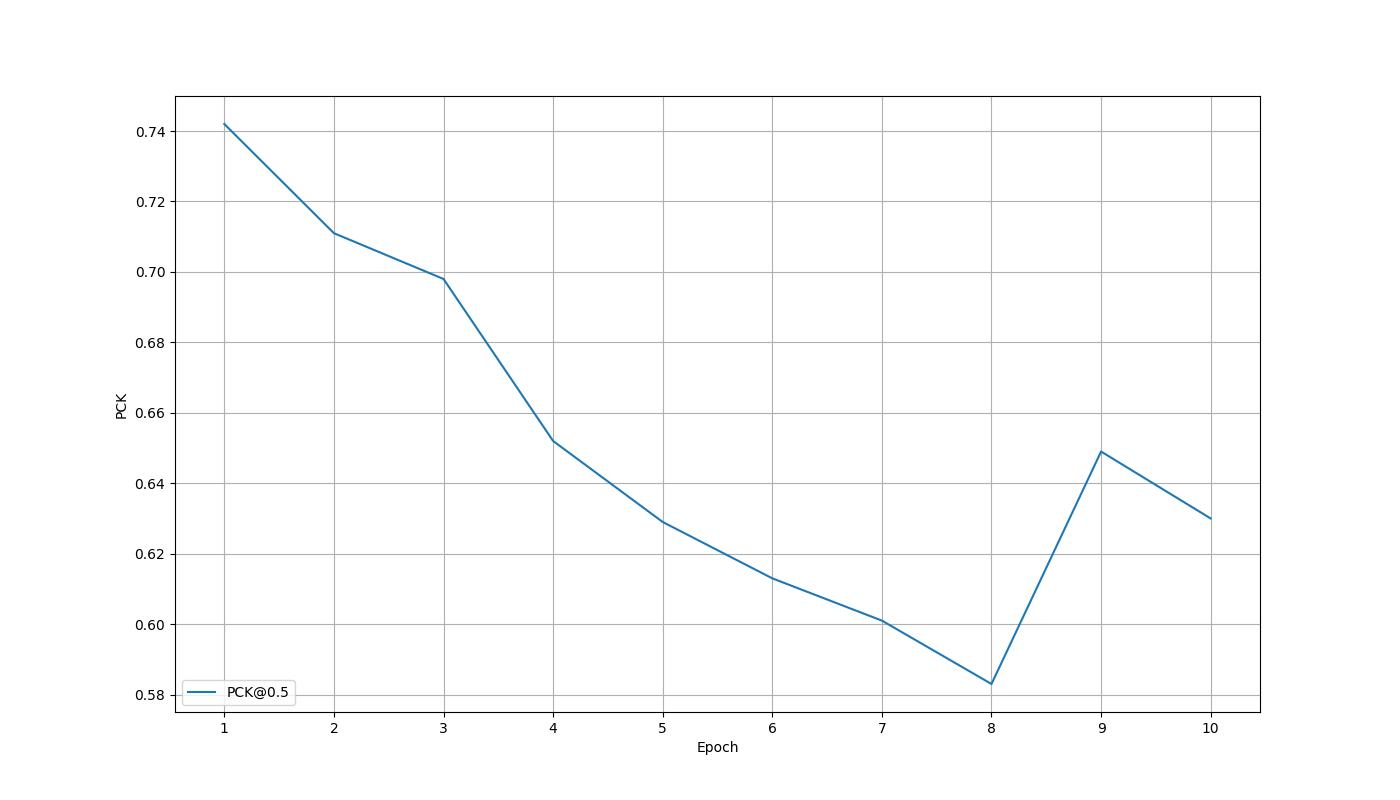
\includegraphics[width=\textwidth]{./images/results/hrnet_pck}
	\caption{Зависимость метрики PCK на целевом домене от номера итерации.}
	\label{fig:hrnet_pck}
\end{figure}

Для данной модели эксперимент признан неудачным, поэтому другие метрики сниматься не будут. При дальнейших ислледованиях значение порога будет выставляться не ниже 0.5.

\subsubsection*{ViTPose}

С учетом опыта предыдущей модели выбран наиболее высокий возможный порог уверенности равный 0,7. В данном случае модель быстро достигла полной выборки предложенных данных. Так как в рамках эксперимента среди маркеров остановки не было объема выборки, то было проведено все 10 итераций. Как видно на \autoref{fig:vitpose_pck}, наилучшее значение метрики наблюдается на 4 номере итерации. Именно это состояние и будем рассматривать наилучшим в рамках данного эксперимента.

\begin{figure}[h]
	\centering
	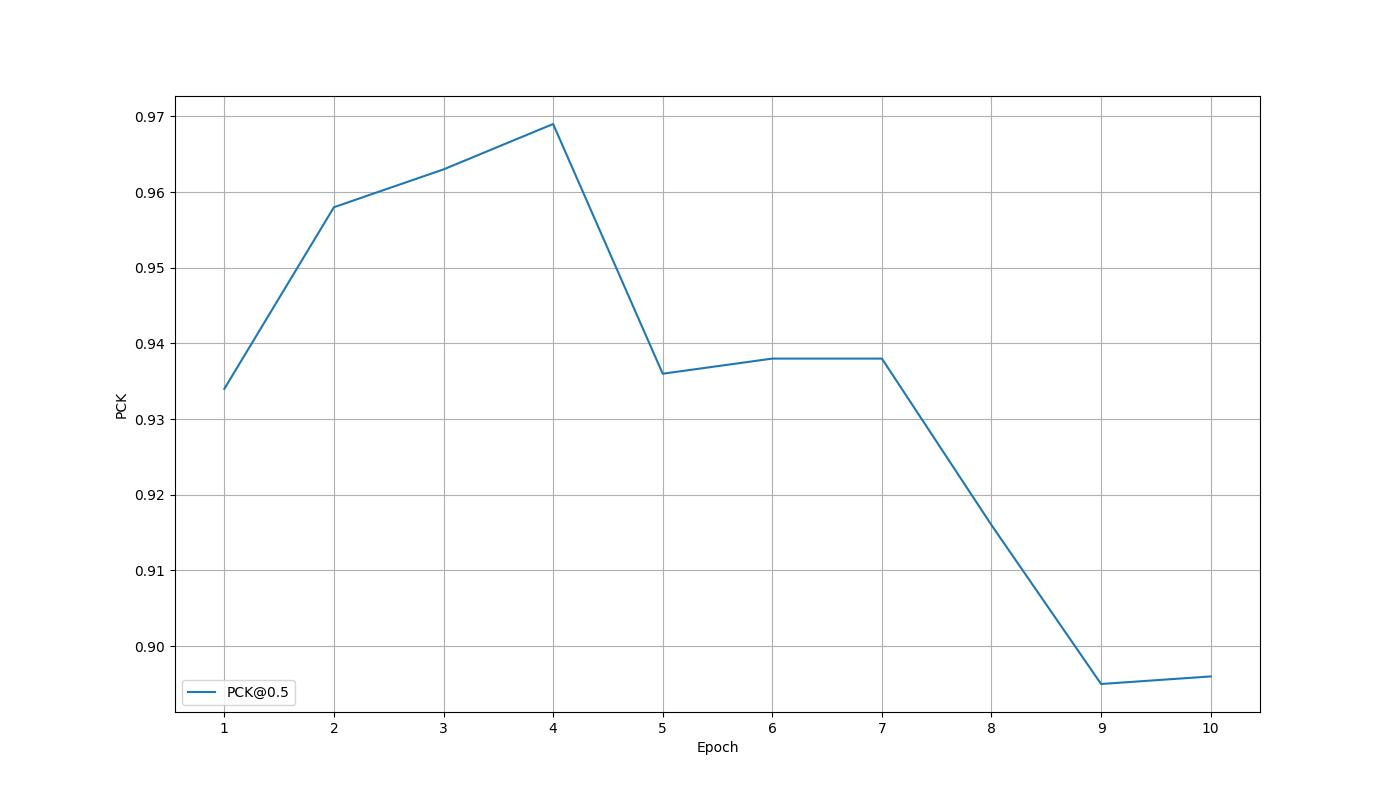
\includegraphics[width=\textwidth]{./images/results/vitpose_pck}
	\caption{Зависимость метрики PCK на целевом домене от номера итерации.}
	\label{fig:vitpose_pck}
\end{figure}

Для полноты картины базовое состояние было обучено на полностью размеченных данных из адаптационной части целевого домена. 

\begin{table}[h]
	\centering
	\begin{tabular}{|p{4cm}||p{2.2cm}|p{2.2cm}|p{2cm}|p{2.2cm}|p{2cm}|p{2cm}|}
		\hline
		&PCK@0.05&PCK@0.25&PCK@0.5\\\hline
		\hline
		Базовое состояние & 0.356 & 0.928 & 0.983\\
		\hline
		Адаптированая модель & 0.144 & 0.539 & 0.745\\
		\hline
		Дообученная на целевом домене  & 0.04 & 0.052 & 0.2\\
		\hline
	\end{tabular}
	\caption{Сравнительная статистика нескольких состояний.}
	\label{tab:vitpose_table}
\end{table}

\subsubsection*{SimCC}

Появится позже

\subsubsection*{RTMPose}

Появится позже

\newpage